\section{问题三：通信约束下的运输与中继联合调度}

\subsection{通信链路模型}

问题三在运输维度上叠加通信保障：运输无人机在爬升、巡航、下降及物资投送阶段须保持连续通信，直连不可用时由中继无人机接力。本文建立"地形遮挡 + 传播损耗 + 双向链路预算"的通信可行性判定模型\cite{ref_itu,ref_zeng,ref_zhan}。

\subsubsection{地形遮挡判定}

对任意两个通信端点，沿其三维视线连线对 30\,m DEM 逐点采样，比较地面高程与两端插值的直线高度，全程不穿地即无遮挡；记遮挡指示变量
\begin{equation}
b_{ijt}=
\begin{cases} 0, & \text{端点 }i,j\text{ 间无地形遮挡},\\ 1, & \text{存在地形遮挡}. \end{cases}
\end{equation}

\subsubsection{双向链路预算}

接收端 $b$ 的有效接收门限由接收灵敏度 $P^{\rm sens}_b$ 与衰落裕量 $M_b$ 共同确定：$P^{\rm th}_b=P^{\rm sens}_b+M_b$。方向 $a\to b$ 的最大允许传播损耗为
\begin{equation}
L^{a\to b}_{\max} = P^{a}_t + G^{a}_t + G^{b}_r - L_{\rm sys} - P^{\rm th}_b,
\end{equation}
其中 $P_t$、$G_t$、$G_r$ 分别为发射功率、发射天线增益、接收天线增益，$L_{\rm sys}$ 为系统损耗。因运输控制与状态回传均需通信保障，主体间按双向链路判定，门限取两方向较小值：$L^{a\leftrightarrow b}_{\max}=\min(L^{a\to b}_{\max},L^{b\to a}_{\max})$。

\subsubsection{传播损耗与链路可用性}

端点 $i,j$ 在 $t$ 时刻的自由空间传播损耗（ITU-R P.525）\cite{ref_itu}为
\begin{equation}
L_{\rm FSPL,ijt} = 32.44 + 20\log_{10} f + 20\log_{10} D_{ijt},
\end{equation}
其中 $f$ 为载波频率（MHz）、$D_{ijt}$ 为三维直线距离（km）。考虑遮挡后的总损耗 $L_{\rm path,ijt}=L_{\rm FSPL,ijt}+L_{\rm obs}\,b_{ijt}$，双向链路可用性定义为
\begin{equation}
A_{ijt}=\begin{cases}1,& L_{\rm path,ijt}\le L^{i\leftrightarrow j}_{\max},\\ 0,& \text{否则}.\end{cases}
\end{equation}

运输无人机在任一时刻的通信状态：与 G01 链路可用时记为\textbf{直连}；直连不可用但"运输—中继"接入链路与"中继—G01"回传链路同时可用时记为\textbf{中继}；其余记为\textbf{通信中断}。中继仅支持单跳，接入与回传链路须同时刻可用。

\subsubsection{中继能耗与候选网格}

中继能耗采用"功率 $\times$ 时长"模型（附件给中继的是功率参数而非航程包线字段）。中继无人机由 O01 起飞、爬升至悬停高度、完成建链后悬停服务、服务结束后下降返航，其架次能耗为
\begin{equation}
E^{\rm relay} = P^{\rm cruise}\cdot t^{\rm cruise} + E^{\rm up}(h,m^{\rm to}) + \bigl(P^{\rm hover}+P^{\rm comm}\bigr)\cdot t^{\rm hover},
\end{equation}
其中 $P^{\rm cruise}$ 为巡航功率、$t^{\rm cruise}$ 为水平巡航时间；爬升附加能耗 $E^{\rm up}(h,m^{\rm to})$ 按重力势能公式计算、质量取计划起飞总质量 $m^{\rm to}$；悬停服务能耗由悬停功率 $P^{\rm hover}$ 与通信附加功率 $P^{\rm comm}$ 之和乘悬停时长 $t^{\rm hover}$ 得到，下降附加能耗按题设取 0。中继架次同样满足返航电量约束。

中继悬停位置离散化为"缺口腿水平连线 5 个分数点 $\times$ 6 档悬停高度（50--300\,m）"的候选网格，对每条需中继路线的缺口腿逐一生成候选点，共 3420 个（位置、高度）组合；单条路线的中继需求最多归并为 2 个（位置、时间窗），对应 2 架中继机身的物理上限，超出则诚实标记为违反。

\subsection{主方案：贪心构造 + 中继覆盖分配}

主方案承接问题二贪心路线（对应代码 \texttt{q3\_2.py}），在其上叠加中继覆盖窗口分配与联合派单仿真，分四步。

\textbf{步骤 1--2（基线 + 贪心合并）}：与问题二主方案完全一致，得到 16 条合并路线（能耗 58.179\,kWh）。

\textbf{步骤 3（通信画像 + 中继候选）}：对 16 条路线逐相位做链路预算判定，需中继相位 586/720；对缺口腿生成中继候选网格（共 3420 个候选点），做集合覆盖贪心分配。

\textbf{步骤 4（联合派单仿真）}：运输与中继共享统一资源仿真引擎，按"紧迫覆盖优先 + 打分函数"排程，中继机 2 架 + 能源组件 6 个构成独立资源池。

主方案结果见表~\ref{tab:q3_dispatch}。16 条路线中直连 3、中继覆盖 13、通信缺口 0，通信中断为 0；三组派单预设完全打平：总能耗 67.387\,kWh（运输 58.179 + 中继 9.208），架次 29（运输 16 + 中继 13），makespan 19379.4\,s（5.38\,h），硬时限违反数 18。

\begin{table}[htbp]
\centering
\caption{问题三主方案结果（均衡预设）}
\label{tab:q3_dispatch}
\small
\begin{tabular}{lc}
\toprule
\textbf{指标} & \textbf{数值} \\
\midrule
运输架次 / 中继架次 & 16 / 13 \\
通信保障方式（直连/中继/缺口） & 3 / 13 / 0 \\
通信中断 & 0 \\
总能耗（运输+中继） & 67.387\,kWh（58.179 + 9.208） \\
联合任务完成时间 $f_2$ & 19379.4\,s（5.38\,h） \\
配送及时性 $f_1$ & 2051542.6 \\
硬时限违反数 & 18 \\
\bottomrule
\end{tabular}
\end{table}

图~\ref{fig:q3_main} 给出主方案的路线与通信覆盖图、地形遮挡剖面示例与联合资源甘特图。由图可见，中继主要服务于地形起伏大、与 G01 无视线通路的路段，联合甘特图显示运输与中继架次在时间轴上交错排布、共享电池与能源组件独立充电。

\begin{figure}[htbp]
\centering
\subfloat[路线与通信覆盖]{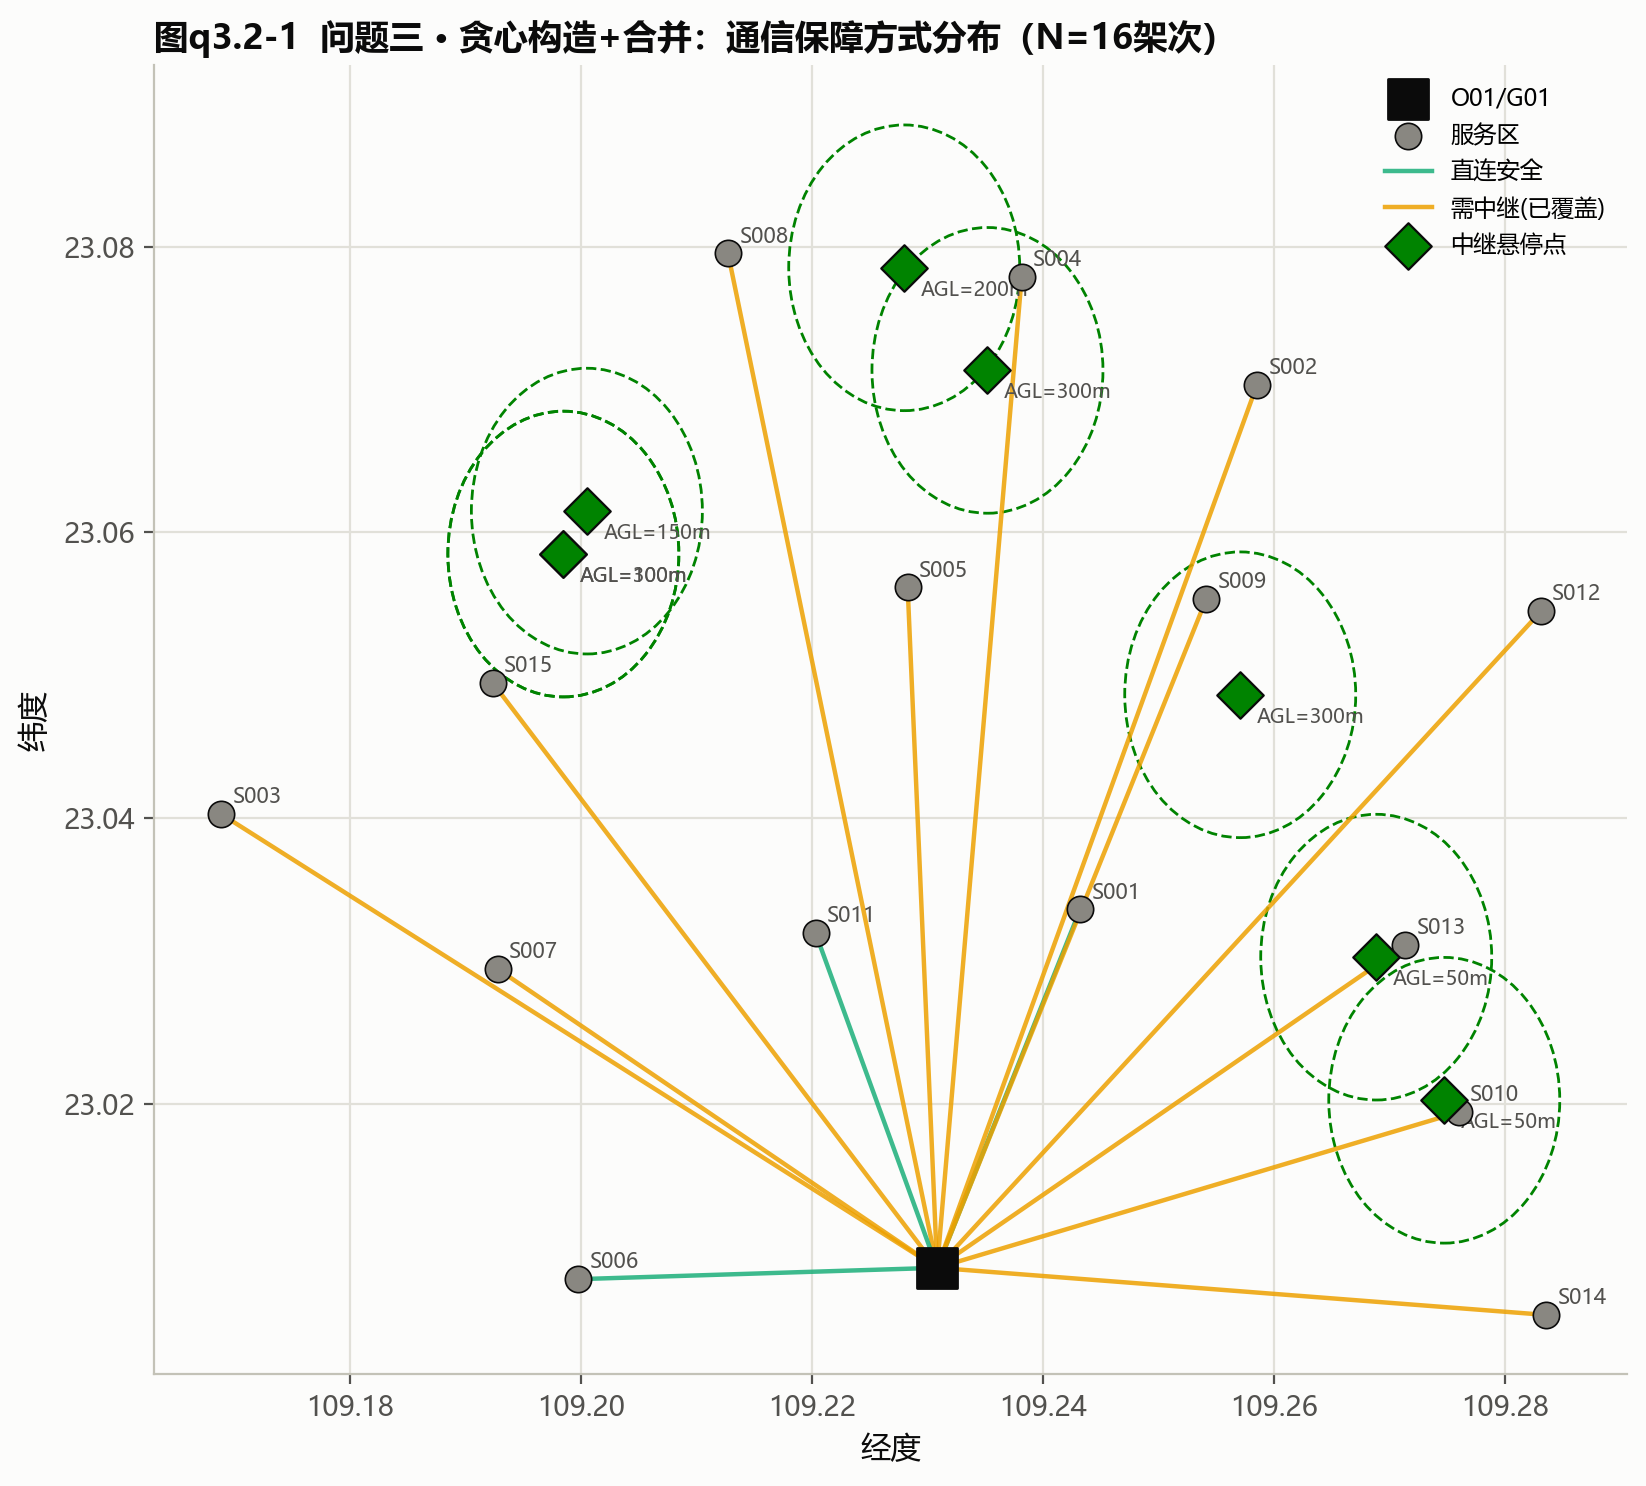
\includegraphics[width=0.48\textwidth]{figures/q3_2_01_路线结构与通信覆盖图.png}\label{fig:q3_main}}
\hfill
\subfloat[联合资源甘特图]{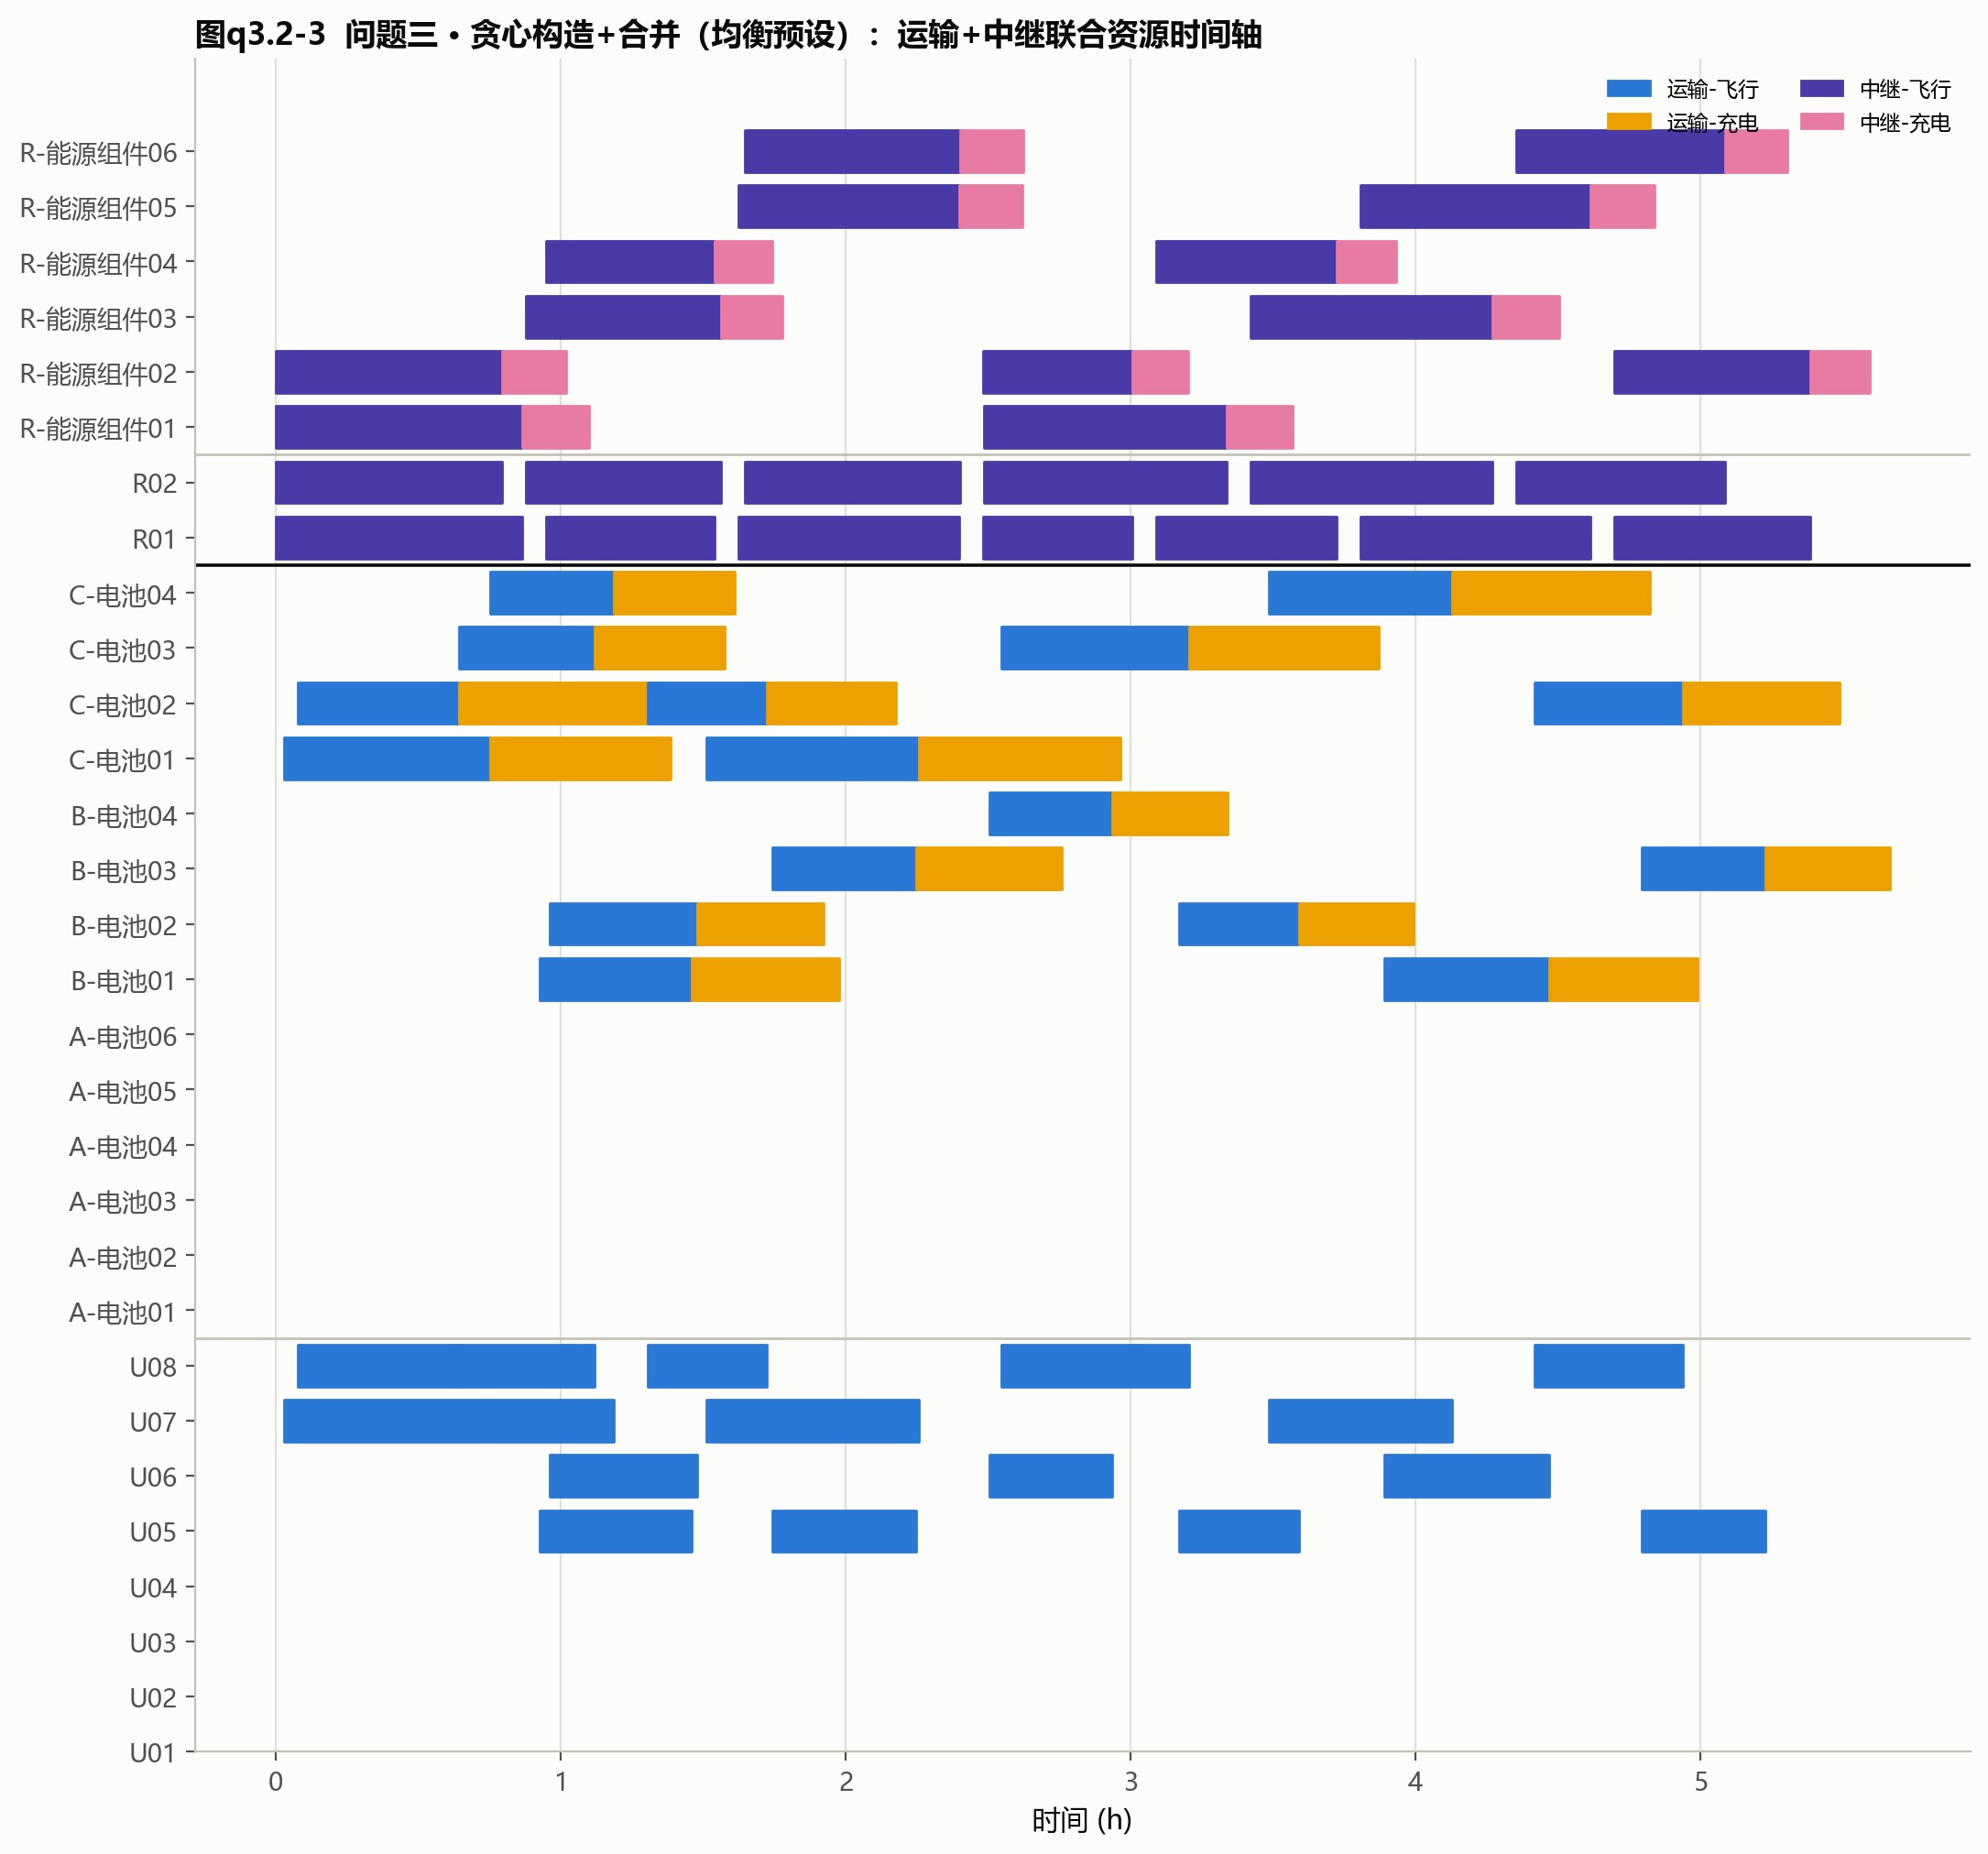
\includegraphics[width=0.48\textwidth]{figures/q3_2_03_联合资源甘特图.png}\label{fig:q3_main_gantt}}
\caption{问题三主方案路线通信覆盖与联合排程}
\label{fig:q3_main_overview}
\end{figure}

图~\ref{fig:q3_main_energy} 展示机队架次与能耗构成，可见中继能耗占总能耗约 13.7\%（9.208/67.387），是叠加通信保障后的合理增量。

\begin{figure}[htbp]
\centering
\subfloat[地形遮挡剖面示例]{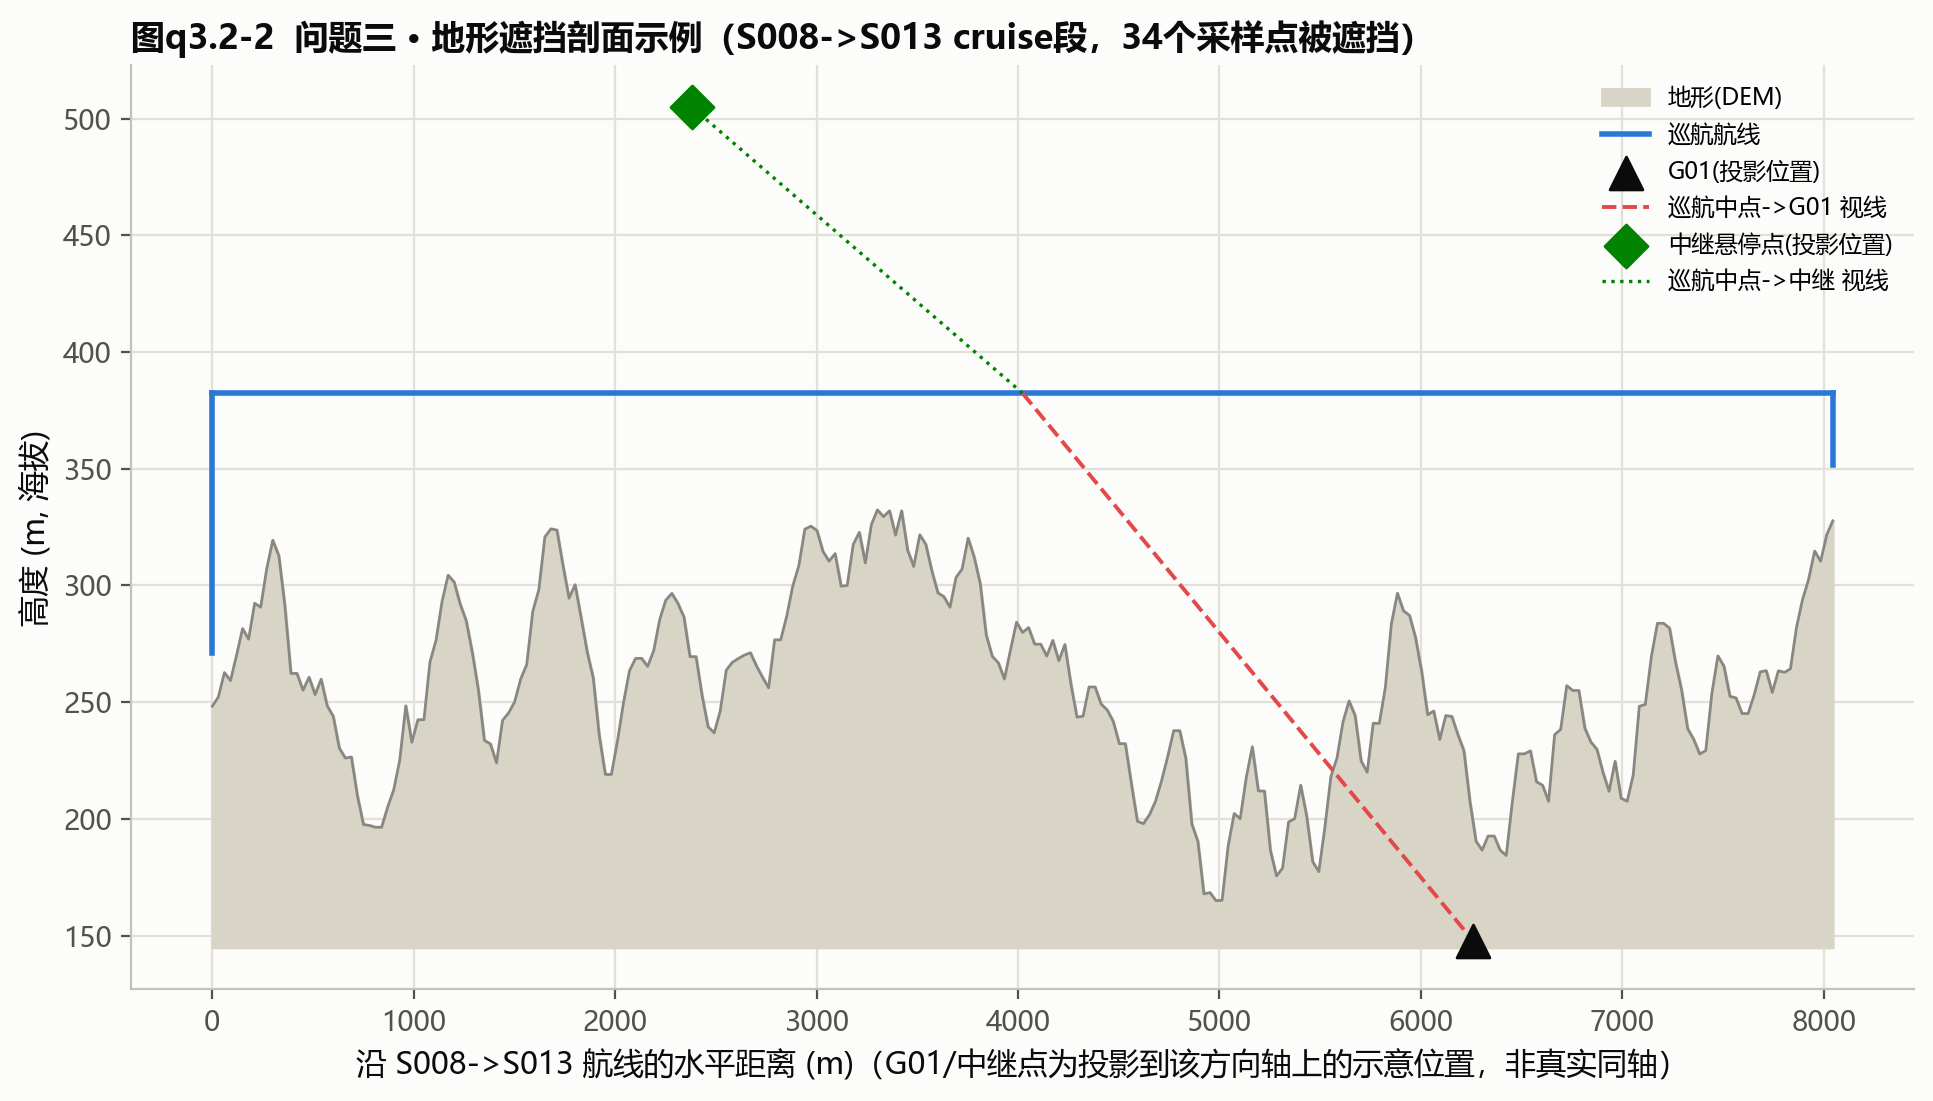
\includegraphics[width=0.48\textwidth]{figures/q3_2_02_地形遮挡剖面示例.png}\label{fig:q3_main_profile}}
\hfill
\subfloat[机队架次能耗对比]{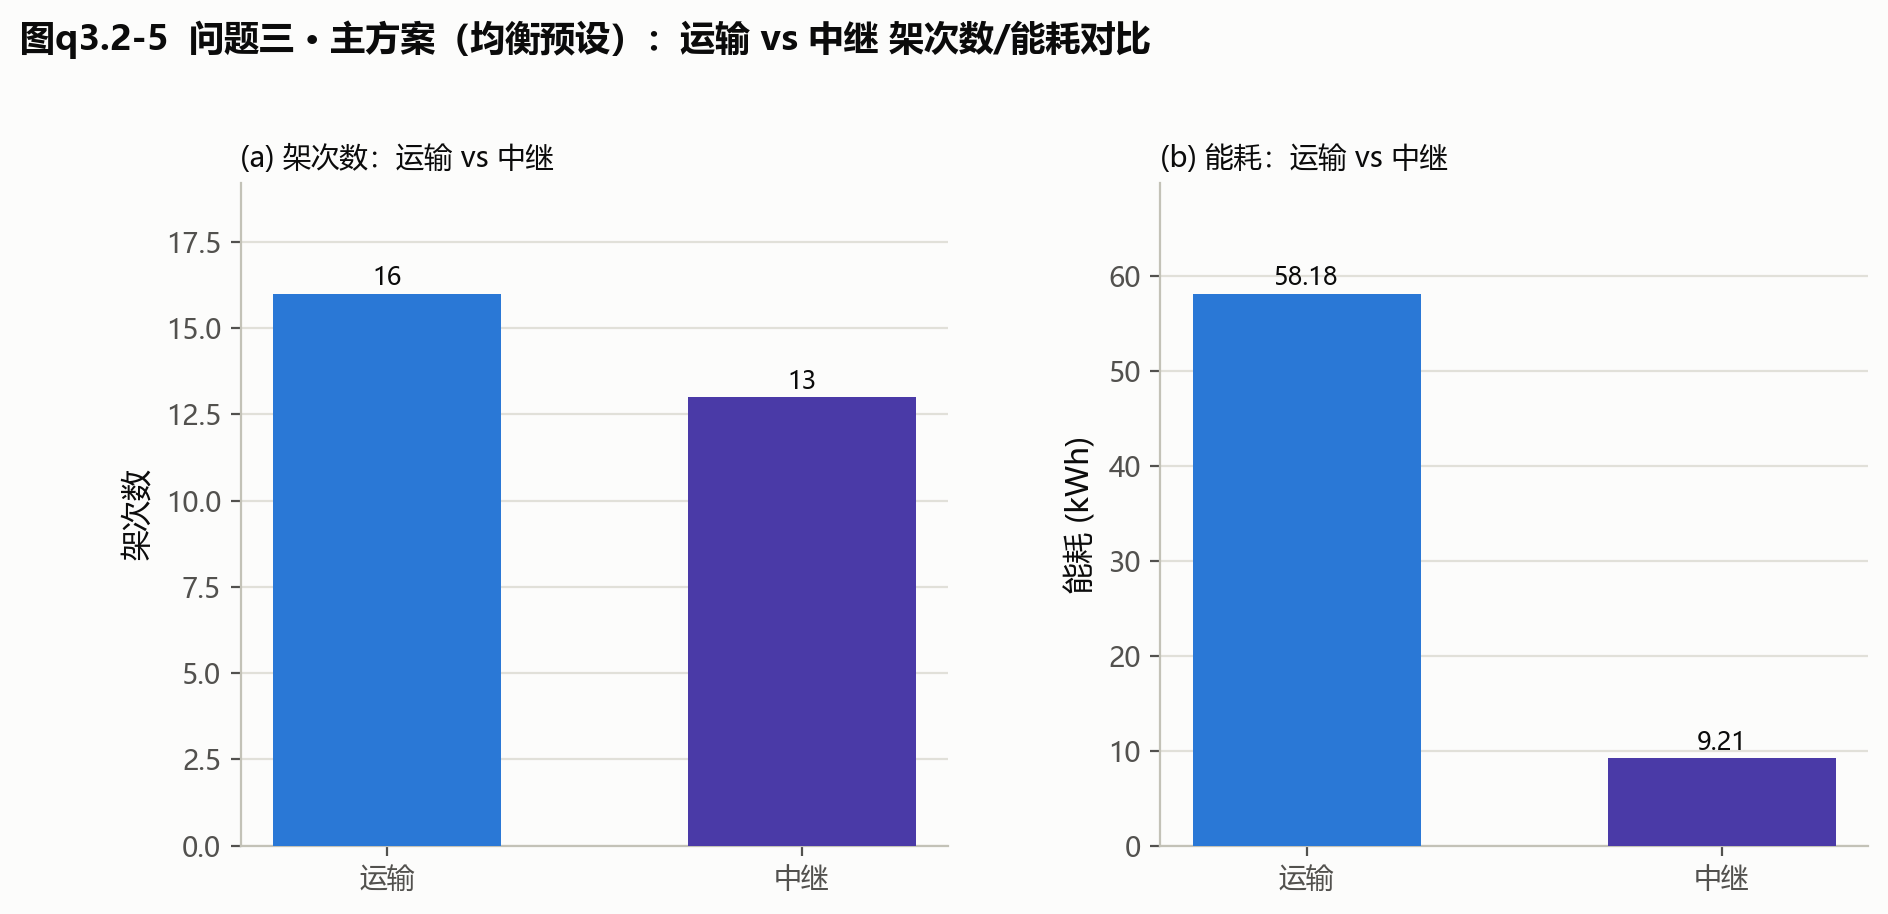
\includegraphics[width=0.48\textwidth]{figures/q3_2_05_机队架次能耗对比.png}\label{fig:q3_main_energy}}
\caption{问题三主方案地形遮挡与能耗构成}
\label{fig:q3_main_energy_overview}
\end{figure}

图~\ref{fig:q3_sankey} 以桑基图直观呈现主方案的能耗与架次流向：总能耗 67.387\,kWh 中运输占 58.179\,kWh（86.3\%）、中继占 9.208\,kWh（13.7\%）；总架次 29 中运输 16、中继 13。中继的能耗与架次占比即为通信保障带来的结构性代价。

\begin{figure}[htbp]
\centering
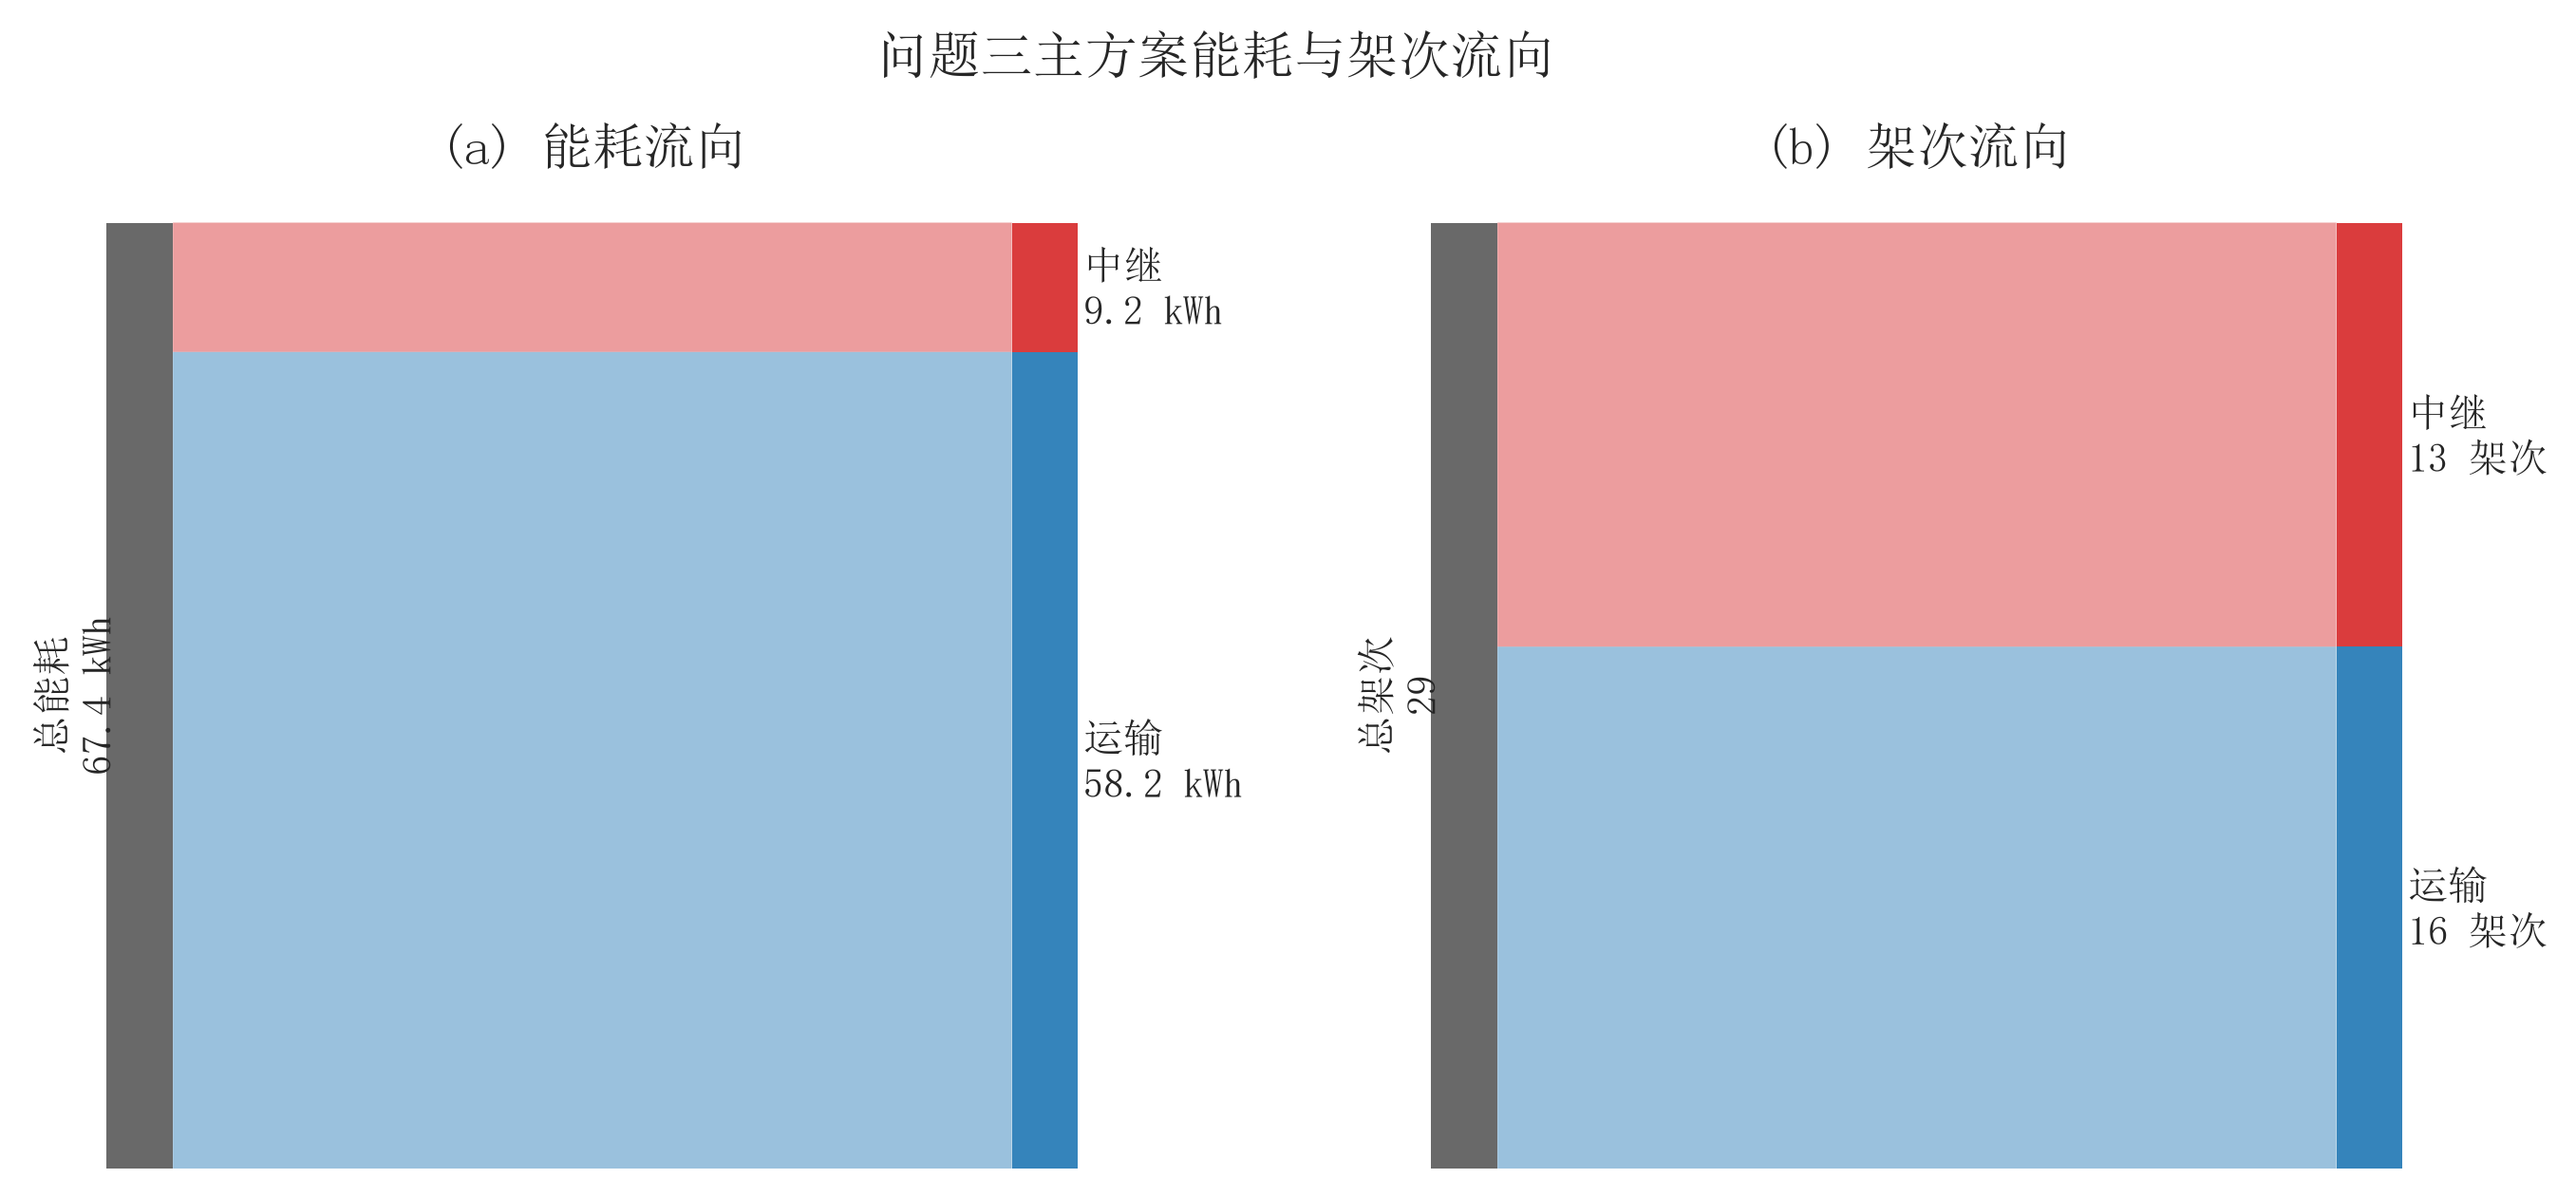
\includegraphics[width=0.95\textwidth]{figures/q3_extra_01_能耗架次Sankey.png}
\caption{问题三主方案能耗与架次流向}
\label{fig:q3_sankey}
\end{figure}

图~\ref{fig:q3_coverage} 对比主方案与对比方法的通信覆盖方式构成，可见两种方法均无通信缺口（中断为 0），区别在于中继覆盖路线的绝对数量——主方案路线少、中继覆盖 13 条，对比方案路线多、中继覆盖 35 条，印证了"中继资源充足即可彻底消除通信盲区"的结论。

\begin{figure}[htbp]
\centering
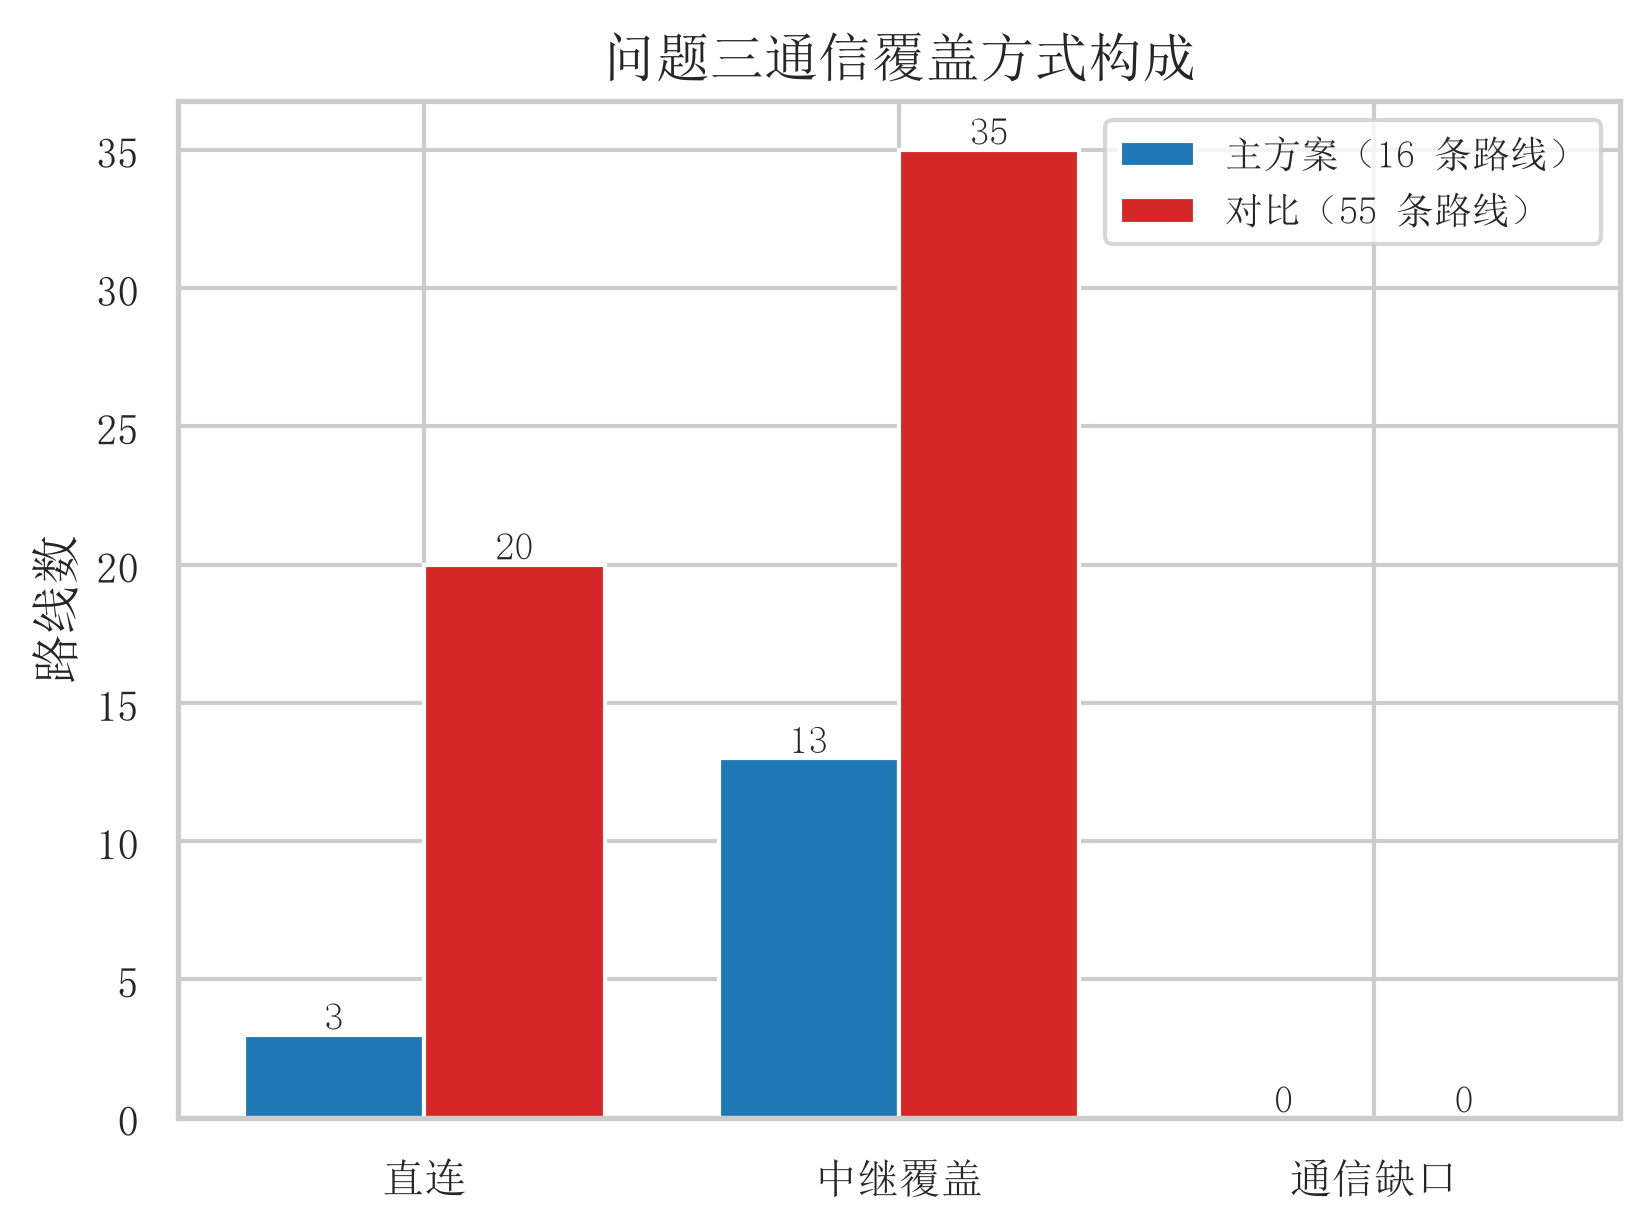
\includegraphics[width=0.6\textwidth]{figures/q3_extra_04_通信覆盖构成.png}
\caption{问题三两种方法通信覆盖方式构成}
\label{fig:q3_coverage}
\end{figure}

\subsection{对比方法：NSGA-II 路线-中继联合优化}

对比方法（对应代码 \texttt{q3\_1.py}）复用问题二 NSGA-II 的全局分组编码，将运输分组染色体与中继位置联合优化（中继位置由确定性函数计算、不参与遗传搜索），目标为 $f_1\sim f_4$ 加违反量。参数：pilot（24、5）+ 正式种群 80、代数 80，变异率 0.05。

对比方法结果：55 条运输路线（直连 20 / 中继 35 / 缺口 0），总能耗 135.639\,kWh（运输 110.856 + 中继 24.782），架次 90（运输 55 + 中继 35），makespan 54352.2\,s（15.10\,h），硬约束违反数 12。图~\ref{fig:q3_nsga} 给出其通信覆盖路线图与联合资源甘特图。

\begin{figure}[htbp]
\centering
\subfloat[通信覆盖与路线]{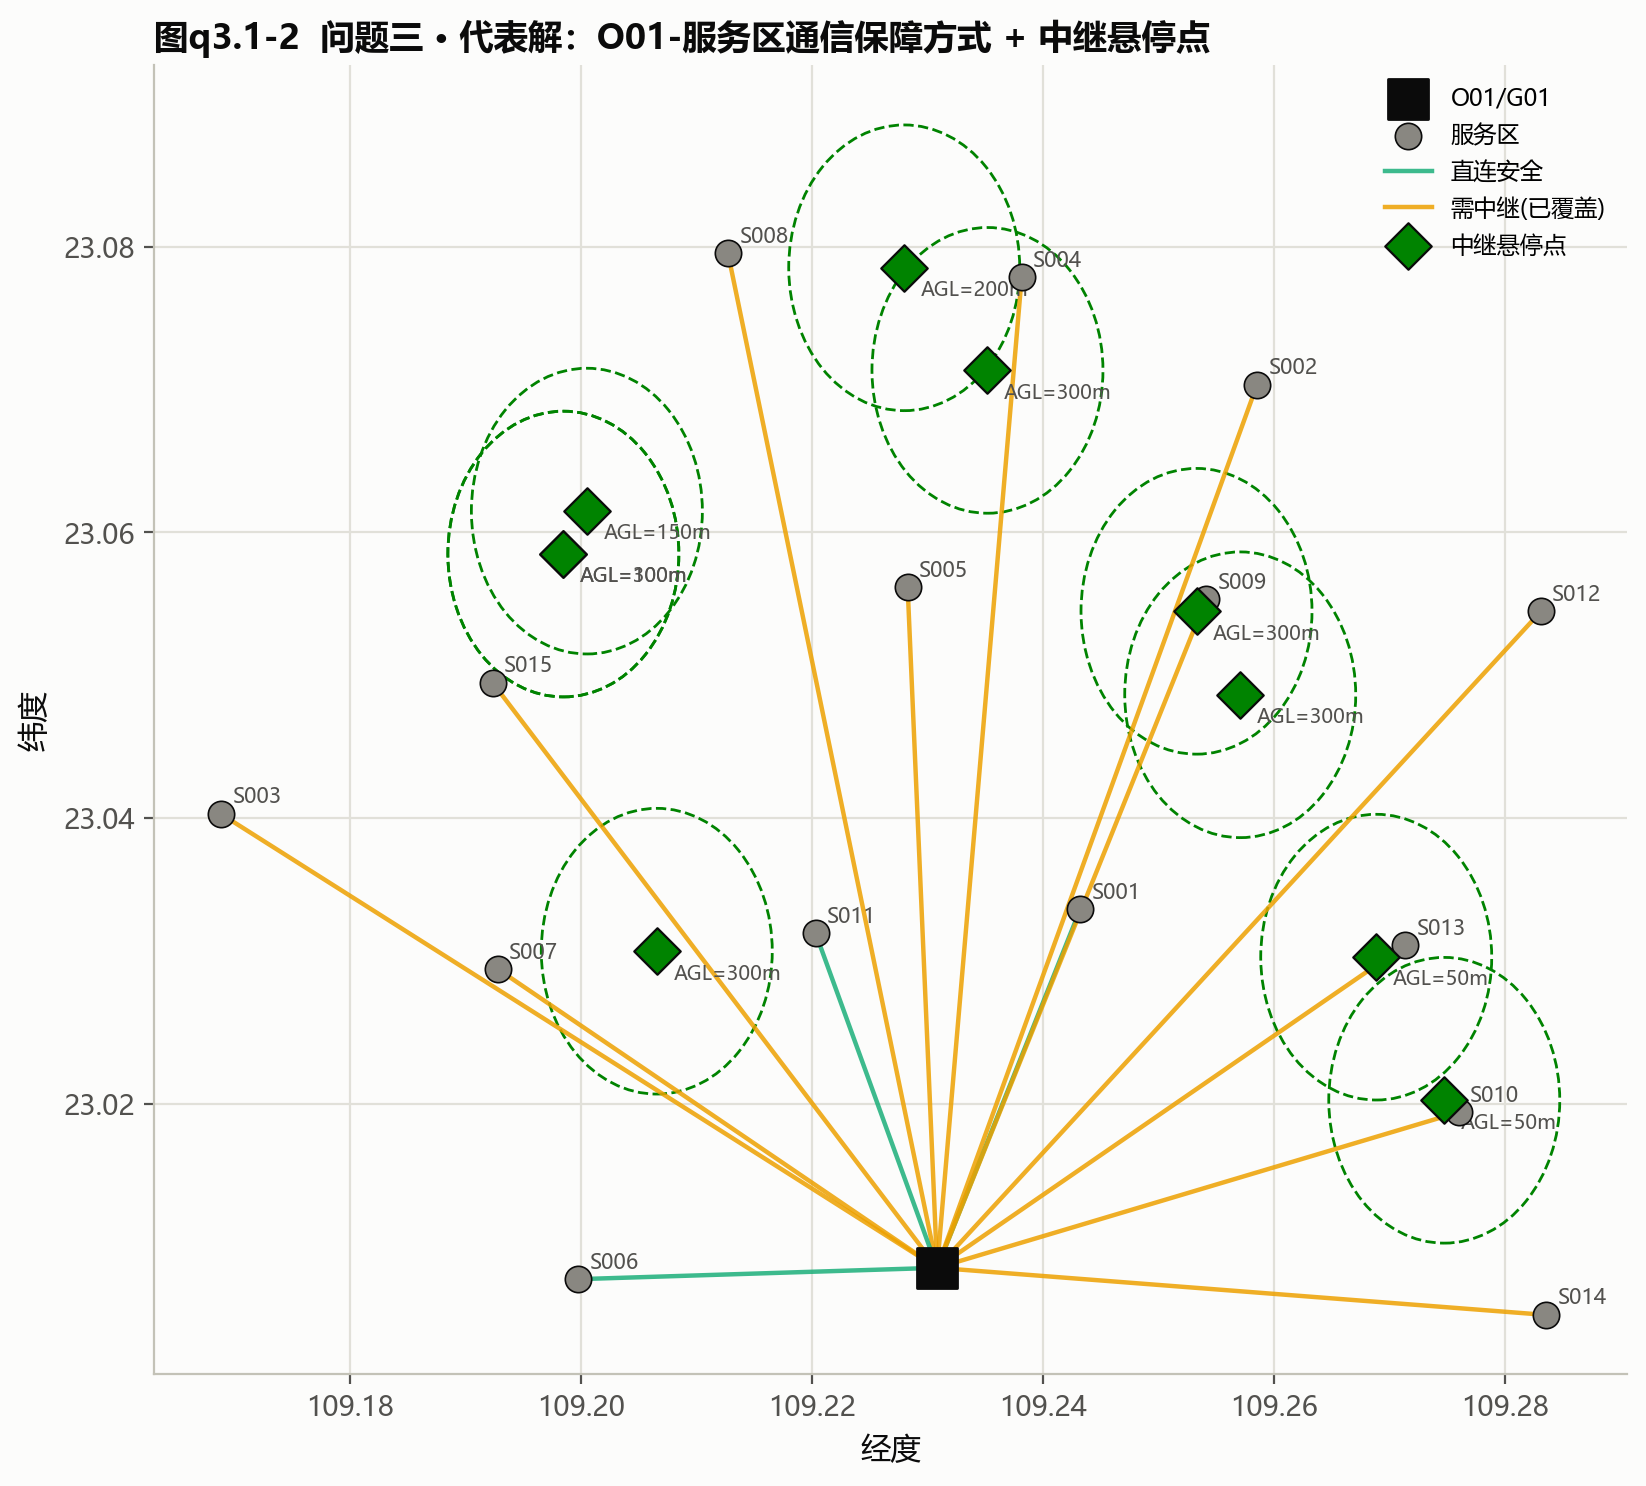
\includegraphics[width=0.48\textwidth]{figures/q3_1_02_通信覆盖与路线图.png}\label{fig:q3_nsga}}
\hfill
\subfloat[联合资源甘特图]{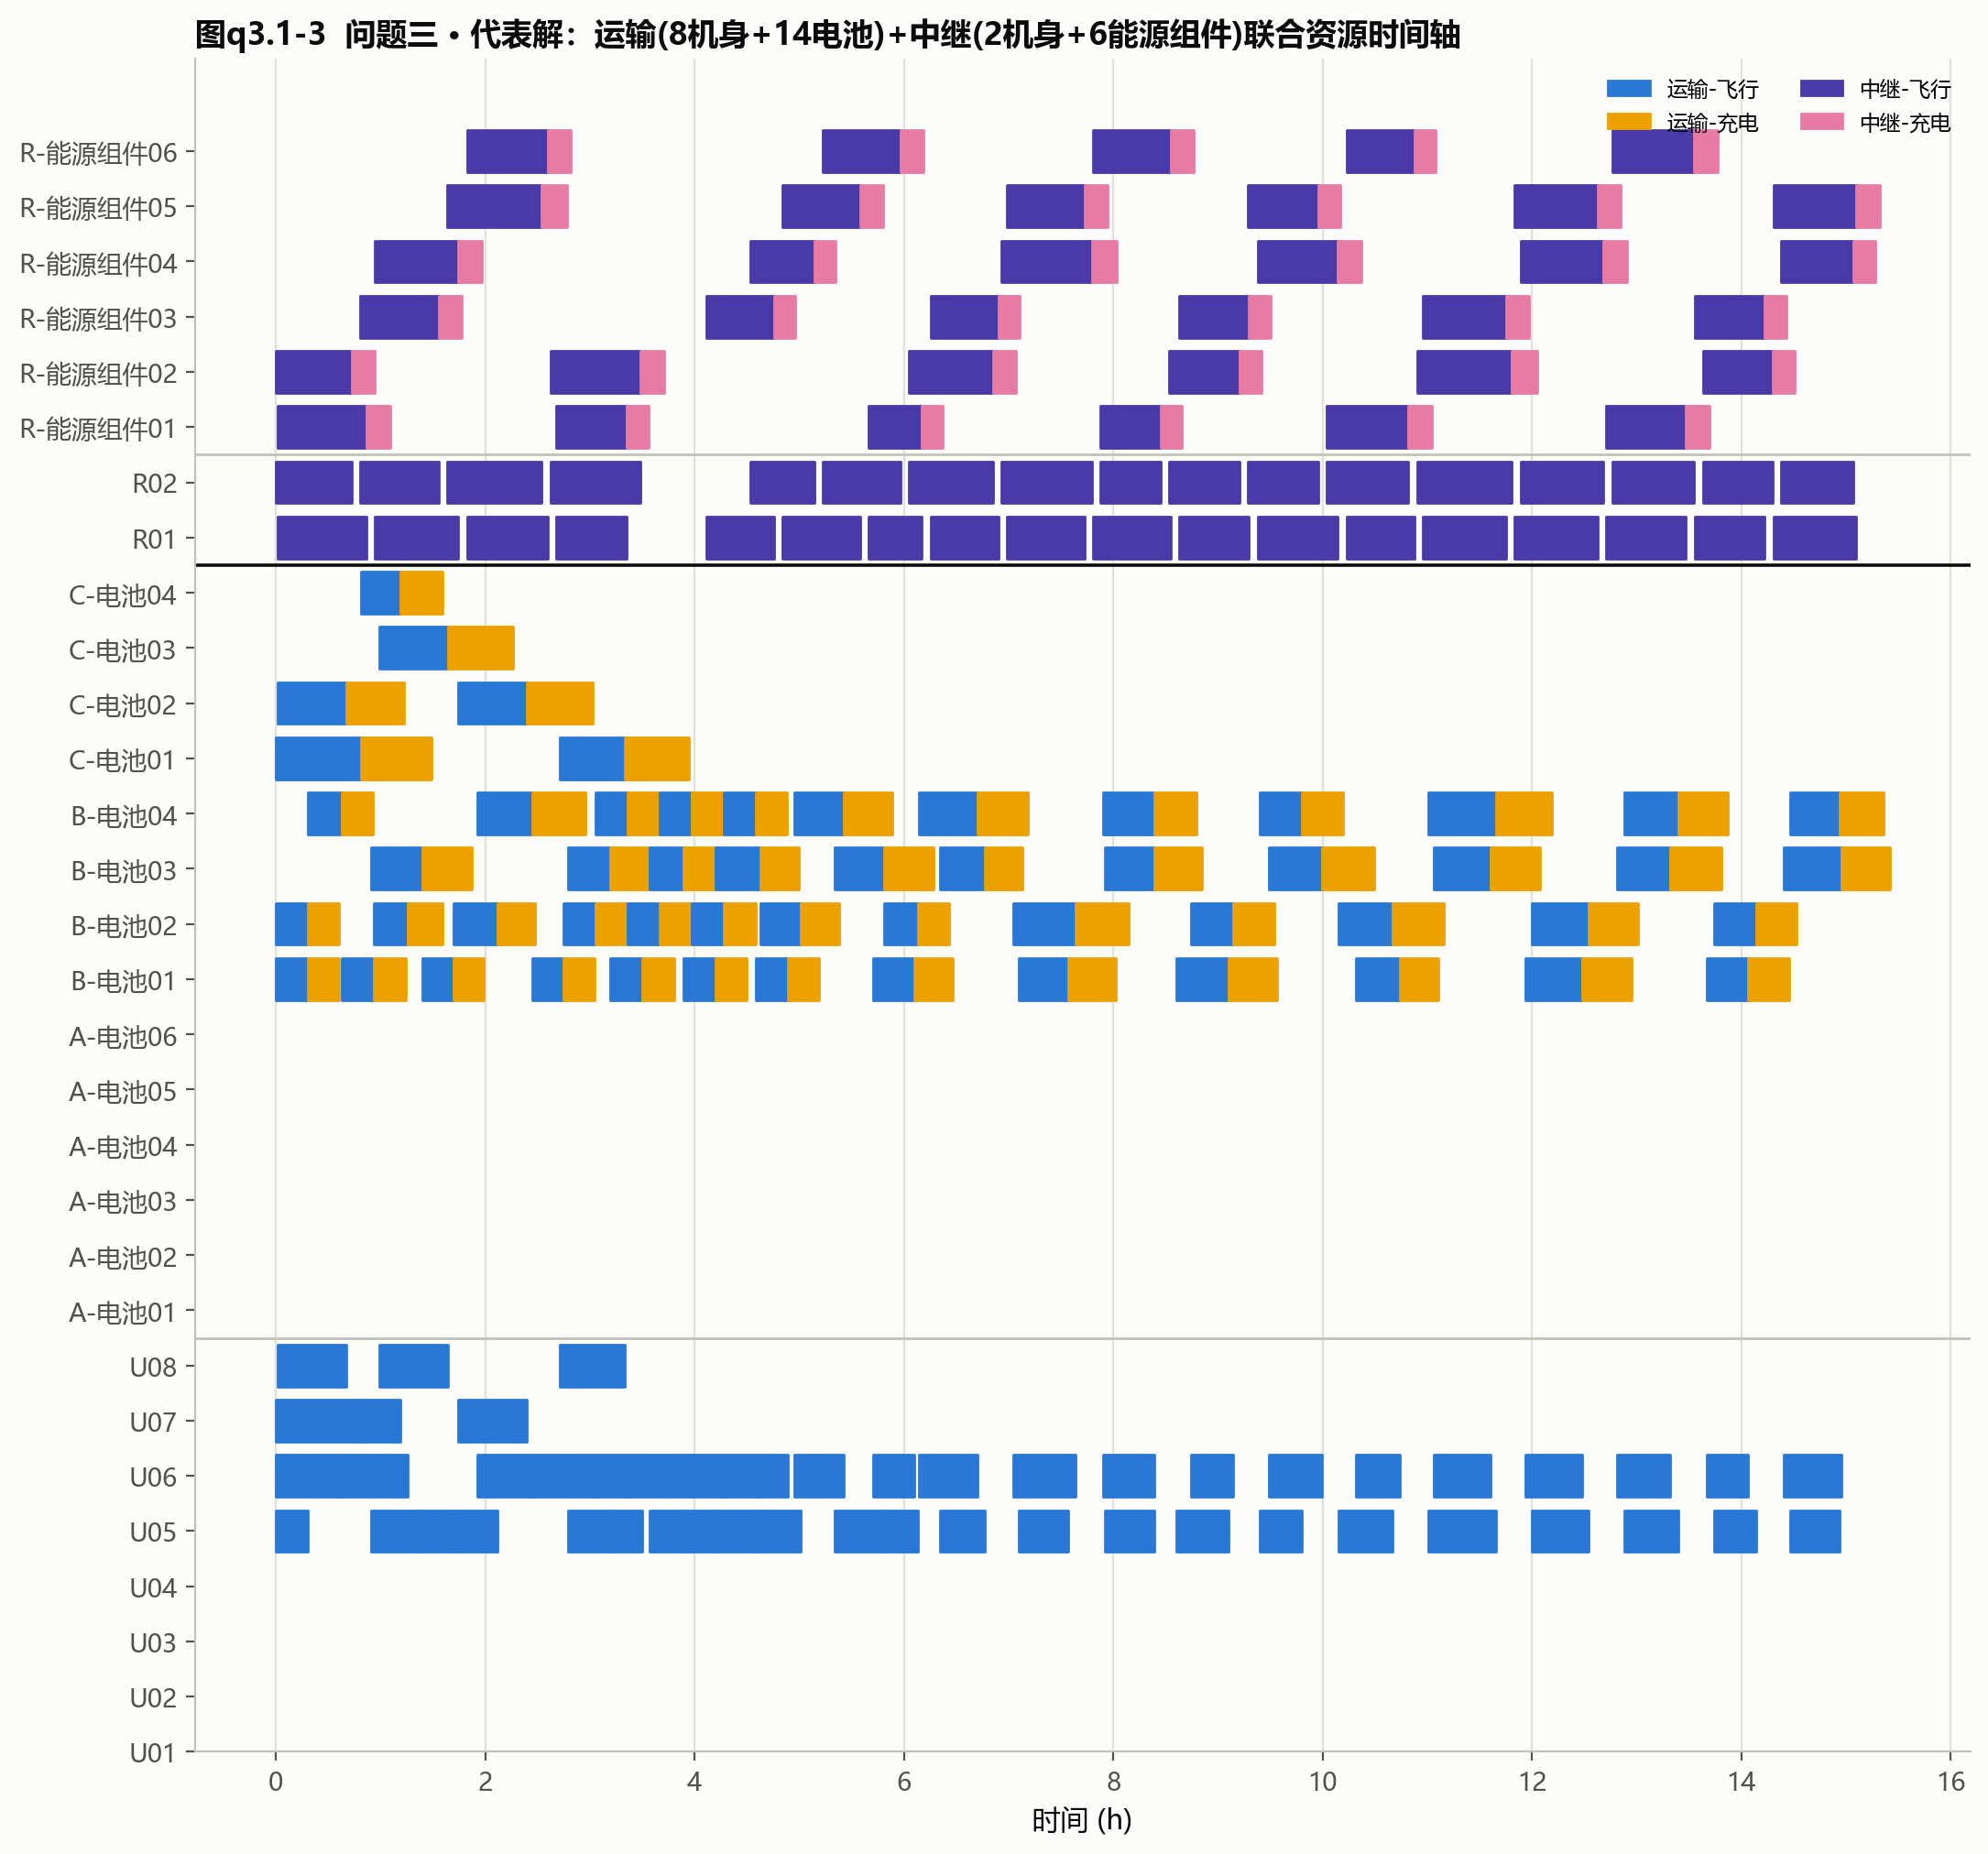
\includegraphics[width=0.48\textwidth]{figures/q3_1_03_联合资源甘特图.png}\label{fig:q3_nsga_gantt}}
\caption{问题三对比方法（NSGA-II 联合优化）结果}
\label{fig:q3_nsga_overview}
\end{figure}

图~\ref{fig:q3_nsga_energy} 给出对比方法的机队架次能耗构成，可见 55 条运输路线的能耗仍以运输为主、中继能耗 24.782\,kWh 占 18.3\%，较主方案的中继占比（13.7\%）更高，印证了"路线越多、需中继覆盖的相位越多、中继能耗占比越高"的规律。

\begin{figure}[htbp]
\centering
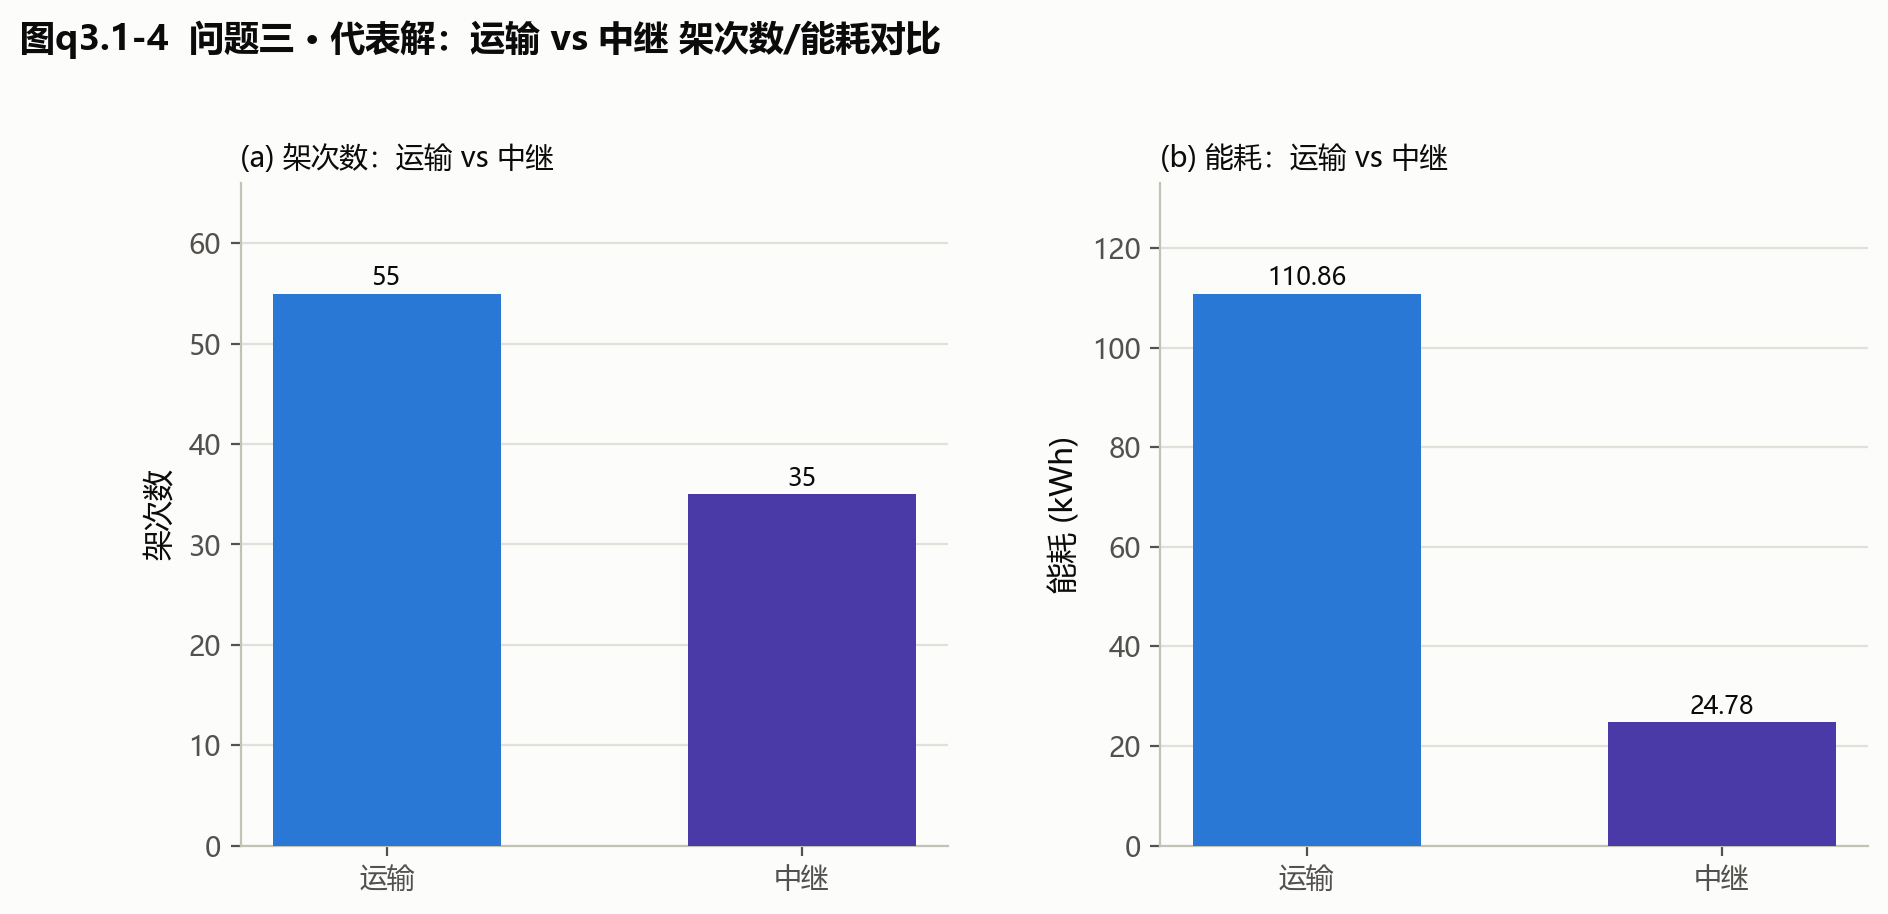
\includegraphics[width=0.62\textwidth]{figures/q3_1_04_机队架次能耗对比.png}
\caption{问题三对比方法机队架次能耗构成}
\label{fig:q3_nsga_energy}
\end{figure}

\subsection{模型比对与通信代价量化}

两种方法对比如表~\ref{tab:q3_compare} 所示。相较问题二（不建模通信）的解，问题三叠加通信保障后必须额外派遣中继架次、消耗额外能量，架次数与总能耗均不低于对应运输分量——这是约束变严格带来的合理代价，而非回归。

\begin{table}[htbp]
\centering
\caption{问题三两种方法及与问题二对比}
\label{tab:q3_compare}
\small
\begin{tabular}{lcccc}
\toprule
\textbf{方案} & \textbf{架次（运+中）} & \textbf{总能耗(kWh)} & \textbf{makespan(s)} & \textbf{硬违约} \\
\midrule
问题二主方案（贪心，无通信） & 16 & 58.179 & 10173.7 & 5 \\
\textbf{问题三主方案（贪心+中继）} & \textbf{29（16+13）} & \textbf{67.387} & \textbf{19379.4} & \textbf{18} \\
问题三对比（NSGA-II 联合） & 90（55+35） & 135.639 & 54352.2 & 12 \\
\bottomrule
\end{tabular}
\end{table}

图~\ref{fig:q3_compare} 给出两种方法在架次、能耗、完成时间、违约四项指标上的直观对比；图~\ref{fig:q3_relay_hover} 给出中继悬停点的高度分布与空间分布，可见中继悬停高度集中于 50--300\,m 的候选网格内、空间上分布在 DEM 起伏较大的路段两侧，与"缺口腿"的通信遮挡判定一致。

\begin{figure}[htbp]
\centering
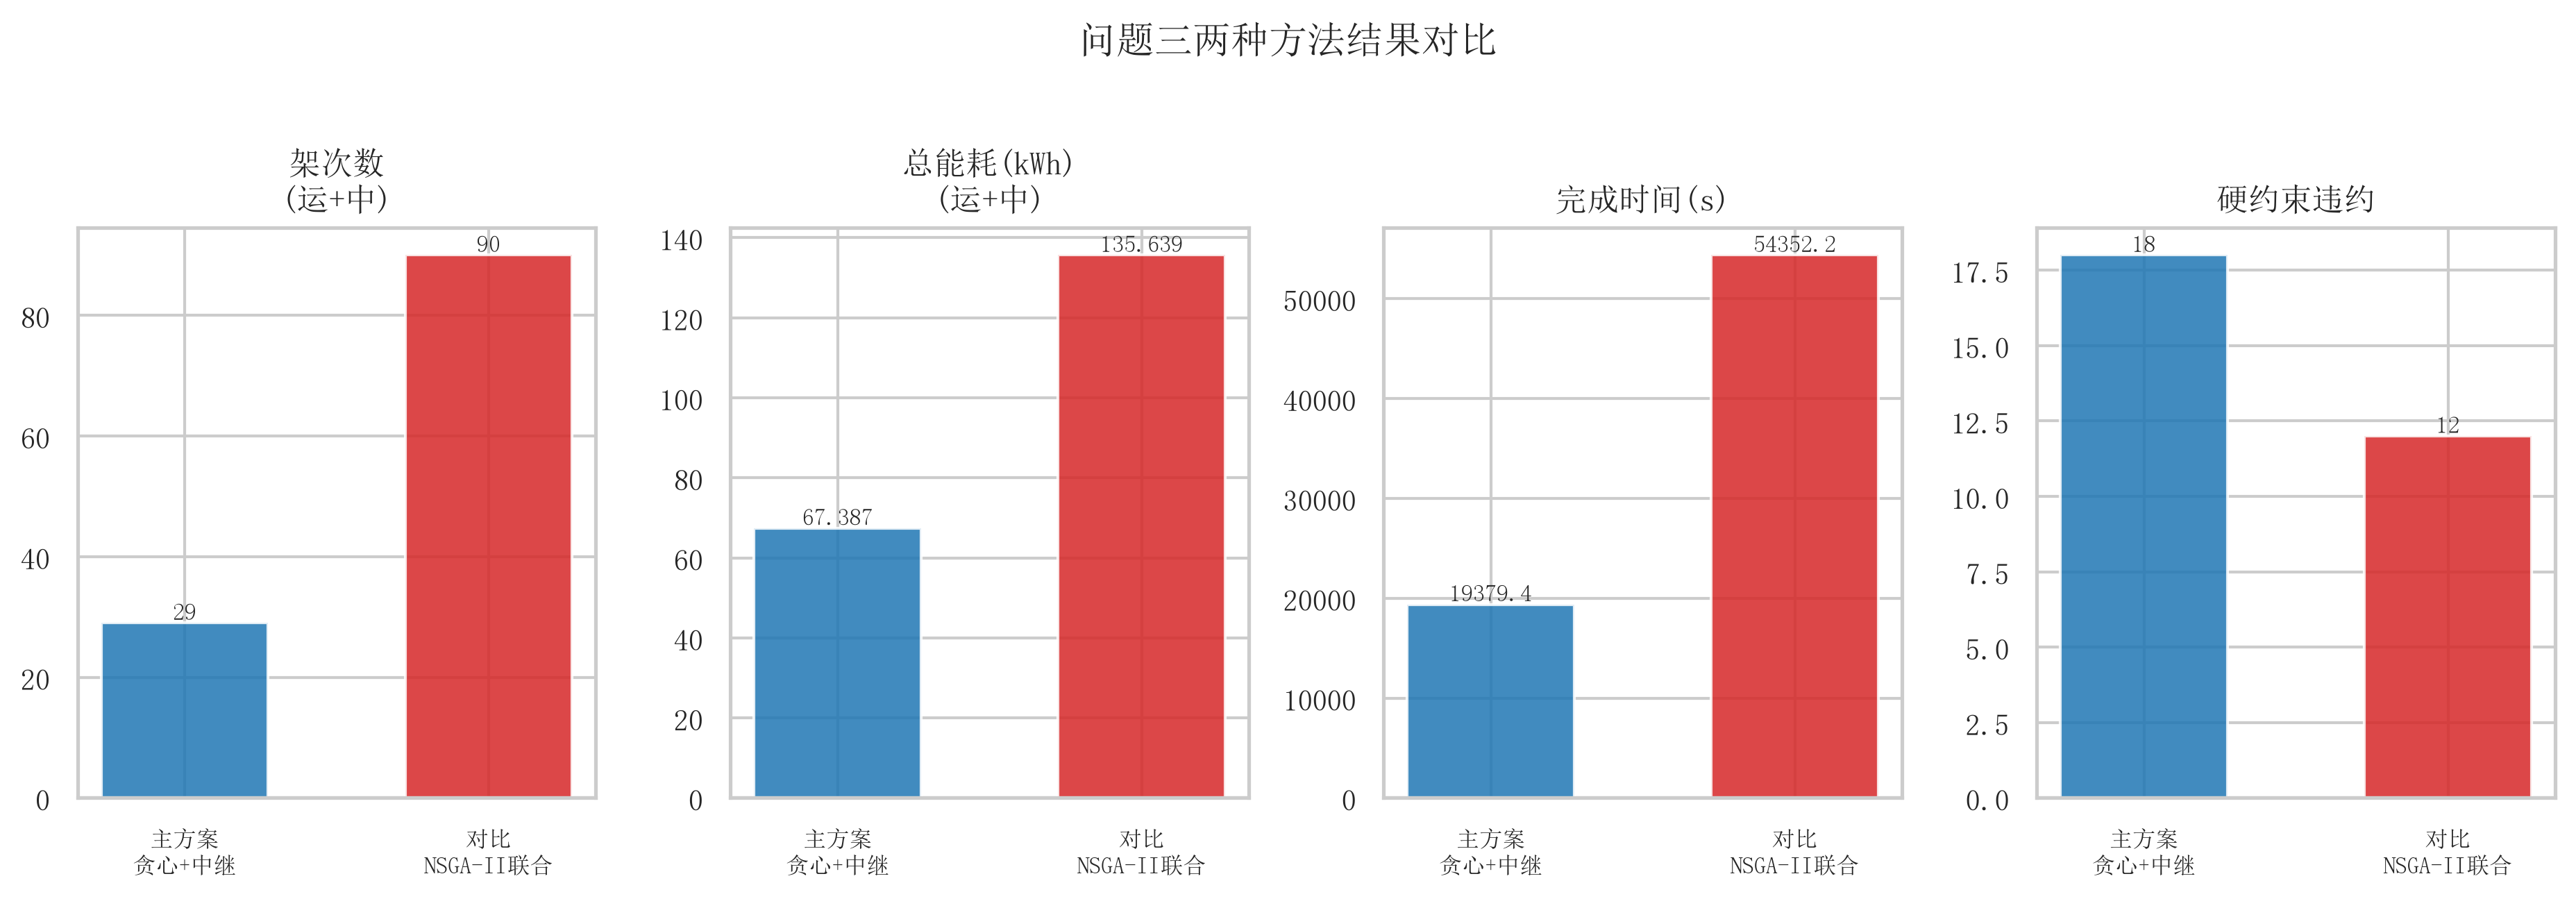
\includegraphics[width=0.95\textwidth]{figures/q3_extra_02_方法对比柱状图.png}
\caption{问题三两种方法四维指标对比}
\label{fig:q3_compare}
\end{figure}

\begin{figure}[htbp]
\centering
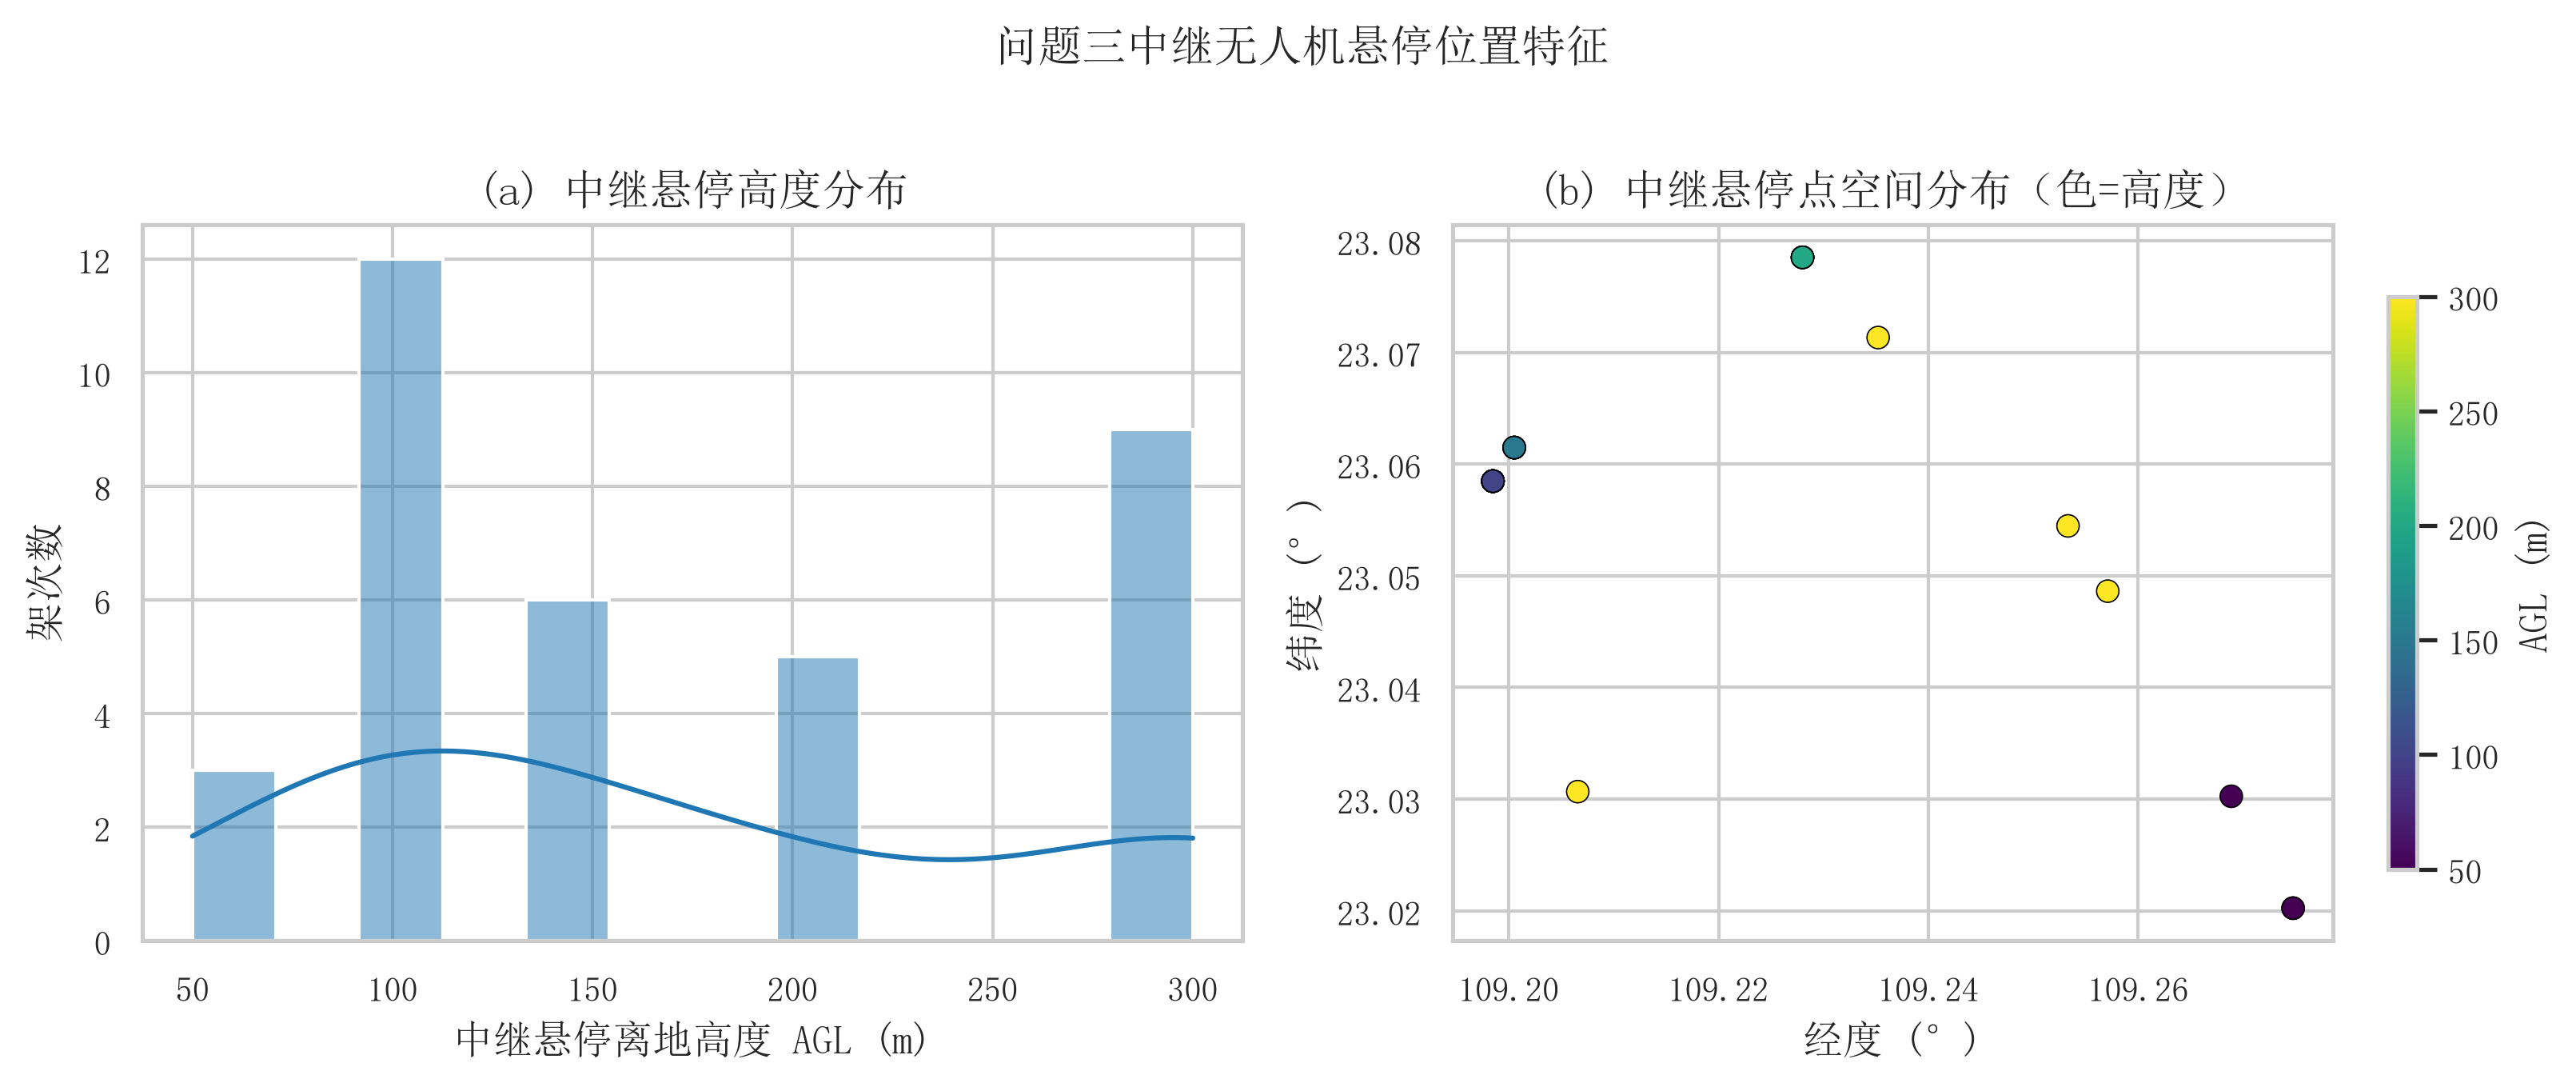
\includegraphics[width=0.95\textwidth]{figures/q3_extra_03_中继悬停特征.png}
\caption{问题三中继无人机悬停位置特征}
\label{fig:q3_relay_hover}
\end{figure}

两种方法均实现了通信中断 0，说明中继覆盖分配在中继资源充足的条件下能彻底消除通信盲区；但叠加中继后硬时限违约进一步上升（贪心路线由 5 增至 18），说明通信保障占用了额外的中继与能源资源、并拉长了部分架次时序，使本就紧的硬时限更难满足。主方案（16 运输 + 13 中继、67.387\,kWh）以更少的资源占用实现同样的通信零中断，作为问题四的承接基准；其中继架次明细见附录~\ref{app:q3_relay}。
